\documentclass[a4paper,12pt]{article}
\usepackage{graphicx}
\usepackage{amsmath}
\usepackage{hyperref}
\usepackage{enumitem}
\usepackage{float}

\title{Events System Documentation}
\author{Bieber Fever}
\date{\today}

\begin{document}

\maketitle
\tableofcontents

\section{Introduction}
\label{sec:introduction}

\section{User Stories / User Characteristics}
\label{sec:user-stories}

\subsection{User Characteristics}

\subsubsection{Host}
Hosts are responsible for organizing, scheduling, and managing events within the organization. 
They create event listings, provide detailed descriptions, set dates, and handle logistics to 
ensure successful execution. Their primary goal is to promote employee bonding, engagement, and 
participation by curating events that are relevant and interesting to employees. They aim to foster 
a sense of community and enhance the workplace culture. Hosts are typically detail-oriented, possess 
strong organizational skills, and have a good understanding of the interests and needs of the employees. 
They should be adept at communication and marketing to effectively promote events. Hosts will require 
tools to manage event details, send invitations, track RSVPs, and gather feedback post-event. They 
will also need access to analytics to assess event success and employee engagement levels. 

\subsubsection{Employee}
Employees are the end-users of the Event System. They browse the events, RSVP to those they are 
interested in, and participate in the activities organized by the Hosts. They aim to find events 
that align with their interests, professional growth, or social engagement needs. Participation 
in these events is expected to enhance their sense of belonging and satisfaction within the organization. 
Employees vary widely in their interests and engagement levels. The system needs to be user-friendly to accommodate 
all employees, regardless of their technical proficiency. Employees will require a calendar view of upcoming events, 
search and filter options to find relevant events, RSVP capabilities, and reminders for events they plan to attend. 
They also need the option to provide feedback on events they attend.

\section{Functional Requirements}
\label{sec:functional-requirements}

\section{Service Contracts}
\label{sec:service-contracts}

\section{Class Diagram}
\label{sec:class-diagram}
\label{sec:class-diagram}
\begin{figure}[H]
    \centering
    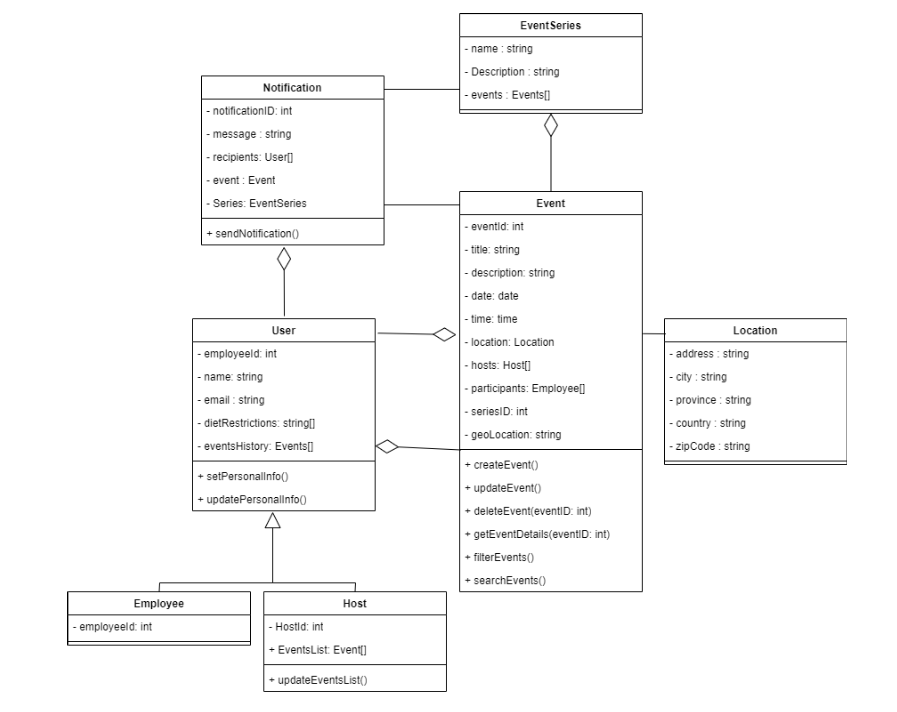
\includegraphics[width=\textwidth]{EventsClassDiagram.png}
    \caption{Class Diagram}
    \label{fig:class-diagram}
\end{figure}

\section{Architectural Requirements}
\label{sec:architectural-requirements}

\subsection{Quality Requirements}
\label{subsec:quality-requirements}

\subsection{Architectural Patterns}
\label{subsec:architectural-patterns}

\subsection{Design Patterns}
\label{subsec:design-patterns}

\subsection{Constraints}
\label{subsec:constraints}

\section{Technology Requirements}
\label{sec:technology-requirements}

\end{document}

